% questions.tex —— 1984 年·全国卷（理科） · 题目内容片段（无答案）
% 由 tools/generate_projects.py 依来源总账自 1984/1984_数学真题_理_试题.md 生成，勿手改（改源 MD 后重跑）


\begin{gktip}
\textbf{来源说明}：本卷为固定原卷《1984理.pdf》单页（原卷页码第 23 页），系 1984 年全国统一招生考试理科卷；同年另有文科卷，二者题目不同。全卷共 20 题，原卷不分节、不设大题号，本库按原卷顺序连续编号为第 1—20 题。原卷未标注分值，题面亦不含答案（答案由本库独立推导）。

\textbf{转录说明}：本代 PDF 的文本层会丢根号与分数线，本文一律按 PDF 页面图像转录；第 1—5 题为选择题（原卷用「（A）（B）（C）（D）」标注），本库统一记为「A．B．C．D．」；第 20 题依原卷配图重绘为 TikZ 矢量图。
\end{gktip}

\begin{question}
\gkti{1}数集 $X=\{(2n+1)\pi,\ n\text{\text{是整数}}\}$ 与数集 $Y=\{(4k\pm1)\pi,\ k\text{\text{是整数}}\}$ 之间的关系是（　）

\begin{gkopts}(4)
\task A．$X\subseteq Y$
\task B．$X\supseteq Y$
\task C．$X=Y$
\task D．$X\ne Y$
\end{gkopts}

\end{question}
\begin{question}
\gkti{2}如果圆 $x^2+y^2+Gx+Ey+F=0$ 与 $x$ 轴相切于原点，那么（　）

\begin{gkopts}(2)
\task A．$F=0,\ G\ne0,\ E\ne0$
\task B．$E=0,\ F=0,\ G\ne0$
\task C．$G=0,\ F=0,\ E\ne0$
\task D．$G=0,\ E=0,\ F\ne0$
\end{gkopts}

\end{question}
\begin{question}
\gkti{3}如果 $n$ 是正整数，那么 $\dfrac18\left[1-(-1)^n\right]\,(n^2-1)$ 的值（　）

\begin{gkopts}(2)
\task A．一定是零
\task B．一定是偶数
\task C．是整数但不一定是偶数
\task D．不一定是整数
\end{gkopts}

\end{question}
\begin{question}
\gkti{4}$\arccos(-x)$ 大于 $\arccos x$ 的充分条件是（　）

\begin{gkopts}(2)
\task A．$x\in(0,1]$
\task B．$x\in(-1,0)$
\task C．$x\in[0,1]$
\task D．$x\in\left[0,\dfrac\pi2\right]$
\end{gkopts}

\end{question}
\begin{question}
\gkti{5}如果 $\theta$ 是第二象限角，且满足 $\cos\dfrac\theta2-\sin\dfrac\theta2=\sqrt{1-\sin\theta}$，那么 $\dfrac\theta2$（　）

\begin{gkopts}(2)
\task A．是第一象限角
\task B．是第三象限角
\task C．可能是第一象限角，也可能是第三象限角
\task D．是第二象限角
\end{gkopts}

\end{question}
\begin{question}
\gkti{6}已知圆柱的侧面展开图是边长为 $2$ 与 $4$ 的矩形，求圆柱的体积。

\end{question}
\begin{question}
\gkti{7}函数 $\log_{0.5}(x^2+4x+4)$ 在什么区间上是增函数？

\end{question}
\begin{question}
\gkti{8}求方程 $(\sin x+\cos x)^2=\dfrac12$ 的解集。

\end{question}
\begin{question}
\gkti{9}求 $\left(|x|+\dfrac{1}{|x|}-2\right)^3$ 的展开式中的常数项。

\end{question}
\begin{question}
\gkti{10}求 $\lim\limits_{n\to\infty}\dfrac{1-2^n}{3^n+1}$ 的值。

\end{question}
\begin{question}
\gkti{11}要排一张有 $6$ 个歌唱节目和 $4$ 个舞蹈节目的演出节目单，任何两个舞蹈节目不得相邻，问有多少种不同的排法（只要求写出式子，不必计算）。

\end{question}
\begin{question}
\gkti{12}设 $H(x)=\begin{cases}0,&x\leqslant0\\1,&x>0\end{cases}$，画出函数 $y=H(x-1)$ 的图象。

\end{question}
\begin{question}
\gkti{13}画出极坐标方程 $(\rho-2)\left(\theta-\dfrac\pi4\right)=0\ (\rho>0)$ 的曲线。

\end{question}
\begin{question}
\gkti{14}已知三个平面两两相交，有三条交线。求证：这三条交线交于一点或互相平行。

\end{question}
\begin{question}
\gkti{15}设 $c$，$d$，$x$ 为实数，$c\ne0$，$x$ 为未知数。讨论方程 $\log_{\left(cx+\frac dx\right)}x=-1$ 在什么情况下有解，有解时求出它的解。

\end{question}
\begin{question}
\gkti{16}设 $p\ne0$，实系数一元二次方程 $z^2-2pz+q=0$ 有两个虚数根 $z_1$，$z_2$。再设 $z_1$，$z_2$ 在复平面内的对应点是 $Z_1$，$Z_2$。求以 $Z_1$，$Z_2$ 为焦点且经过原点的椭圆的长轴的长。

\end{question}
\begin{question}
\gkti{17}求经过定点 $M(1,2)$，以 $y$ 轴为准线，离心率为 $\dfrac12$ 的椭圆的左顶点的轨迹方程。

\end{question}
\begin{question}
\gkti{18}在 $\triangle ABC$ 中，$\angle A$，$\angle B$，$\angle C$ 所对的边分别为 $a$，$b$，$c$，且 $c=10$，$\dfrac{\cos A}{\cos B}=\dfrac ba=\dfrac43$，$P$ 为 $\triangle ABC$ 的内切圆上的动点。求点 $P$ 到顶点 $A$，$B$，$C$ 的距离的平方和的最大值与最小值。

\end{question}
\begin{question}
\gkti{19}设 $a>2$，给定数列 $\{x_n\}$，其中 $x_1=a$，$x_{n+1}=\dfrac{x_n^2}{2(x_n-1)}\ (n=1,2,\cdots)$。求证：

（1） $x_n>2$，且 $\dfrac{x_{n+1}}{x_n}<1\ (n=1,2,\cdots)$；

（2） 如果 $a\leqslant3$，那么 $x_n\leqslant2+\dfrac{1}{2^{n-1}}\ (n=1,2,\cdots)$；

（3） 如果 $a>3$，那么当 $n\geqslant\dfrac{\lg\dfrac a3}{\lg\dfrac43}$ 时，必有 $x_{n+1}<3$。

\Needspace{0.4\textheight}
\end{question}
\begin{question}
\gkti{20}如图，已知圆心为 $O$、半径为 $1$ 的圆与直线 $L$ 相切于点 $A$，一动点 $P$ 自切点 $A$ 沿直线 $L$ 向右移动时，取弧 $\widehat{AC}$ 的长为 $\dfrac23 AP$，直线 $PC$ 与直线 $AO$ 交于点 $M$。又知当 $AP=\dfrac{3\pi}{4}$ 时，点 $P$ 的速度为 $v$，求这时点 $M$ 的速度。
\nopagebreak[4]
\begin{center}% 1984 年全国卷（理科）第 20 题：半径为 1 的圆与直线 l 相切于 A，动点 P 沿 l 右移，直线 PC 交直线 AO 于 M（按源卷布局）。
% 取坐标 A=(0,0)、圆心 O=(0,1)；图示时刻取弧 AC 对应圆心角 75°，C 落在圆上右下方，M 在 O 上方。
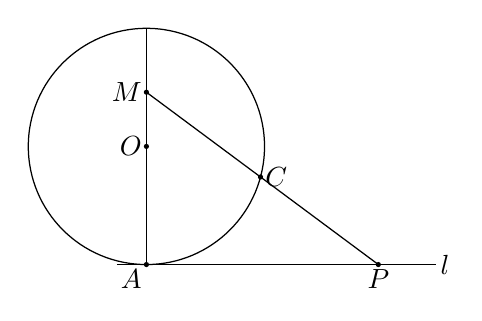
\begin{tikzpicture}[scale=1.5, line width=0.45pt,
  every node/.style={inner sep=1.5pt}]
  \coordinate (A) at (0,0);
  \coordinate (O) at (0,1);
  \coordinate (T) at (0,2);          % 直径上端点
  \coordinate (P) at (1.9635,0);     % 动点 P（在 l 上，A 之右）
  \coordinate (C) at (0.9659,0.7412); % 圆上点 C（弧 AC 长 = 2/3·AP）
  \coordinate (M) at (0,1.4589);     % 直线 PC 与直线 AO 的交点
  \draw (O) circle (1);
  \draw (-0.25,0) -- (2.45,0);       % 切线 l
  \draw (A) -- (T);                  % 直线 AO（过 A 的直径）
  \draw (P) -- (M);                  % 直线 PC（M、C、P 共线）
  \fill (A) circle (0.022);
  \fill (O) circle (0.022);
  \fill (P) circle (0.022);
  \fill (C) circle (0.022);
  \fill (M) circle (0.022);
  \node[left] at (M) {$M$};
  \node[left] at (O) {$O$};
  \node[below left] at (A) {$A$};
  \node[below] at (P) {$P$};
  \node[right] at (C) {$C$};
  \node[right] at (2.45,0) {$l$};
\end{tikzpicture}
\end{center}
\nopagebreak[4]

\end{question}